\part{L'humain se concentre sur les tâches qui nécéssite d'avoir des traits humains}
\chapter{l'Intelligence Artificelle ne peux pas remplacer l'humain pour toutes les tâches}
\section{Intelligence Artificielle Forte}
L'intelligence artificelle forte est l'intelligence
telle qu'elle existe chez l'homme, une somme de procédés cognitifs avancés mais
même aujourd'hui le fonctionnement du cerveau et de l'intelligence reste mystérieuse
et donc la faisabilité d'une IA forte est sans cesse remise en question.

\subsection{Prérequis}
puisque la définition de l'Intelligence elle même reste flou, il est difficile
de donner une liste exacte et correcte des critères pour qu'une IA forte
puisse exprimer une intelligence semblable à celle de l'homme mais
il une liste de critères semble être indéniablement nécéssaires pour remplir
les critères et la majorité des chercheurs en intelligence artificelle semble
s'être mis d'accord sur la liste de critères suivantes: \newline

%TODO approfondir chaque item
\begin{itemize}
    \item Capacité de raisonnement et de jugement:
    \begin{quotation}
    <<Le raisonnement est un processus cognitif permettant
    de poser un problème de manière réfléchie en vue d'obtenir un ou plusieurs résultats.
    L'objectif d'un raisonnement est de mieux cerner (comprendre) un fait ou d'en vérifier la réalité,
    en faisant appel alternativement à différentes « lois » et à des expériences,
    ceci quel que soit le domaine d'application : mathématiques, système judiciaire,
    physique, pédagogie, etc.>>
    \footnote{\url{https://fr.wikipedia.org/wiki/Raisonnement}}
    \end{quotation}

    c'est en somme la capacité à trouver de manière générique la solution à un problème appliqué
    ou abstrait associé à la capacité à utiliser les connaissances nécéssaires pour pouvoir
    résoudre ledit problème.
    \newline

    \item Capacité à conceptualiser ses connaissances: \newline
    Il s'agit d'avoir une IA capable de vider tout "contenu" d'une connaissance et d'en garder
    que l'idée abstraite, la concptualisation des connaissances est essentielle dans l'apprentissage
    et un des principes qui explique le fossé qui sépare le cerveau humain de l'intelligence
    artificelle faible. %TODO peux encore ameliorer cet item
    \newline


    \item Capacité de communication dans un langage naturel: \newline
    La capacité à parler une langue humaine de manière fluide
    tout en comprenant les spécificité du langage mais aussi la sémantique du langage,
    la communication dans un langage naturel est souvent associée à l'intelligence humaine
    et principalement utilisé pour mesurer l'intelligence (test de turing par exemple)
    à cause des processus nécéssaires tel que la représentation mentale, l'empathie,
    la métacognition.
    \newline


    \item Capacité de planification:
    %TODO indiquer
    \begin{quotation}
        <<En intelligence artificielle, la planification automatique
    (automated planning en anglais) ou plus simplement planification, vise à développer des
    algorithmes pour produire des plans typiquement pour l'exécution par un robot ou tout autre agent.
    Les logiciels de planification qui incorporent ces algorithmes s'appellent des planificateurs.
    La difficulté du problème de planification dépend des hypothèses de simplification qu'on tient
    pour acquis, par exemple un temps atomique, un temps déterministe, une observabilité complète, etc.>>
    \footnote{\url{https://fr.wikipedia.org/wiki/Planification_(intelligence_artificielle)}}
    \end{quotation}

    La planification automatique se base sur 3 paramètres d'entrée:
    \begin{itemize}
        \item état de départ
        \item actions possibles
        \item objectif \newline
    \end{itemize}

    \begin{figure}[H]
        \centering
        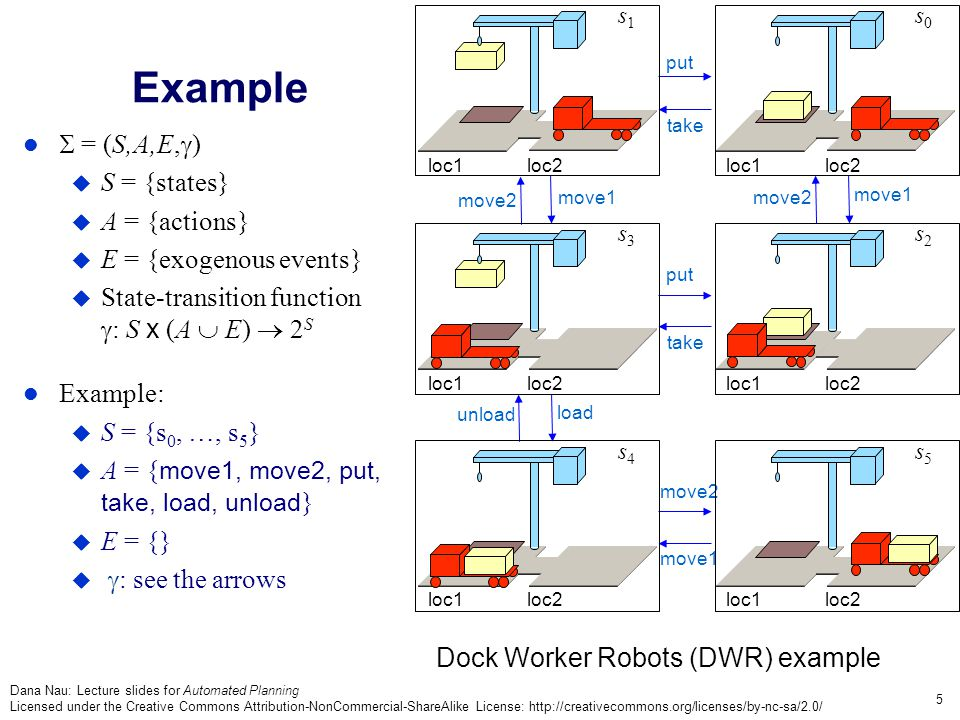
\includegraphics[width=0.7\textwidth]{Images/automatedPlanification}
        \caption{Planification automatique avec un automate}
        \label{fig:chineseroom}
    \end{figure}

    la difficulté de la planification automatique avec une intelligence artificelle forte est dù
    au charactère non-déterministe de la majorité des actions que cette dernière doit réaliser,
    contrairement à un automate ou toutes ses actions sont déterministes, de plus
    la liste des actions possible n'est plus réellement fixe. \newline
\end{itemize}

\subsection*{Freins majeur de la création d'Intelligence Artificelle Forte}
\section{L'experience de pensée "Chinese Room"}
En 1980 John Searle, philosophe américain, publie son article "Minds, Brains, and Programs" dans la revue
scientifique "Behavioral and Brain Sciences" qui donna lieu à de grands débat dans le domaine philosophique
mais surtout dans le domaine de l'intelligence artificelle,
la source de ces débats est une expérience de pensée qui se nomme "Chinese Room". \newline

\begin{figure}[H]
    \centering
    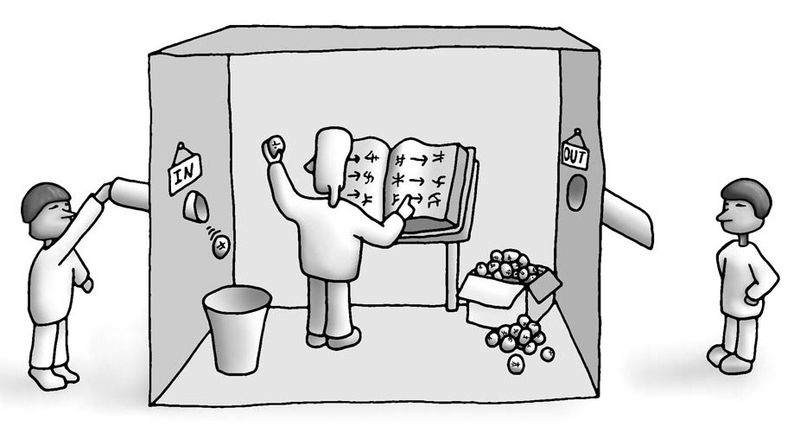
\includegraphics[width=1\textwidth]{Images/chineseroom}
    \caption{Chinese room experiment - wikicommons}
	\label{fig:chineseroom}
\end{figure}

Cette expérience est définie comme suit: \newline
il y a, enfermé dans une piece sans aucun moyen de contact vers l'exterieur, une personne anglophone qui ne comprend
pas le chinois et dans cette piece des boites remplies de symboles chinois ainsi qu'un manuel d'instructions.
Cette personne reçois des symboles chinois envoyé par une personne parlant chinois qui sont en réalité des questions,
dans le manuel d'instruction est indiqué quoi renvoyer en fonction de ce que la personne anglophone reçois,
la personne renvoie des symboles qui sont des réponses à la question reçue, la personne parlant le chinois
pense ainsi parler à une personne qui connaît la langue alors que ce n'est pas le cas.

\begin{figure}[H]
    \centering
    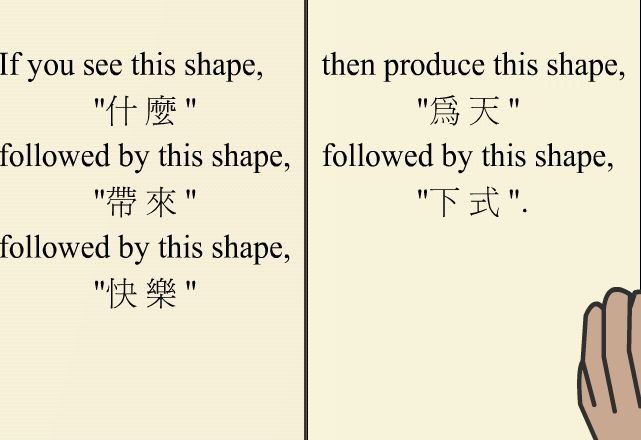
\includegraphics[width=0.7\textwidth]{Images/chineserule}
    \caption{Extrait du manuel d'instruction - David L. Anderson}
	\label{fig:chineseroom}
\end{figure}

l'argument de cette expérience est que meme si la machine répond aux questions qui semble laisser penser
la présence de capacité à penser (une IA forte) elle ne fait en réalité que manipuler des symboles
sans les interpreter (IA faible). \newline

\begin{figure}[h]
    \centering
    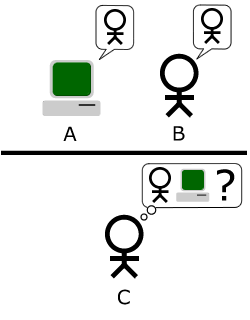
\includegraphics[width=0.3\textwidth]{Images/turingtest}
    \caption{Interprétation basique du test de Turing}
    \label{fig:turingtest}
\end{figure}

l'objectif de cette experience est d'invalider la capacité du test du turing à établir si une
intelligence artificelle a la capacité de penser, le test de turing est une expérience à l'aveugle
ou une personne converse avec un interlocuteur qui est est soit une vrai personne ou un humain
si le sujet avec qui l'IA converse n'est pas capable de detecter qu'il ne parle pas avec un humain mais
une machine cette dernière réussie le test or l'experience chinese room essaie de démonter
justement que la capacité à converser ne va pas forcément prouver l'intelligence et la capacité à penser
car il suffit de manipuler les symboles d'une manière assez complexe pour tromper l'interlocuteur humain.
\newline

En conclusion, l'experience de pensée Chinese room montre qu'avec le type d'ordinateur que
nous avons aujourd'hui il n'est point possible de réaliser d'intelligence artificelle forte
et que nous ne pouvons théoriquement que réaliser des IA qui simulent l'intelligence.

\section{simuler l'intelligence n'est pas encore à la portée de l'IA }

Dans la partie précédente nous avons vu grâce à l'experience de pensée Chinese Room que communiquer
dans un langage naturel de manière indifferentiable d'un humain n'est pas forcément l'expression d'une
intelligence mais qu'en est-il réelement de la performance de l'IA dans la compréhension et l'utilisation
du langage humain ? \newline

De plus le langage, pour la majorité des métiers, n'est qu'un outils pour communiquer. La reconnaissance
d'image, la reconnaissance vocal ne sont que des parties apparentes de ce que doivent résoudre les IA
en terme de problèmes métiers, des choses assez triviales pour nous autres humains, il faut donc se pencher
sur les capacité actuelles de l'IA et la vitesse de son évolution pour établir les domaines
et type de compétences qui pourrait être assimilé assez facilement par l'IA. \newline

\subsection*{Les Assistants Personnels}
\begin{figure}[h]
    \centering
    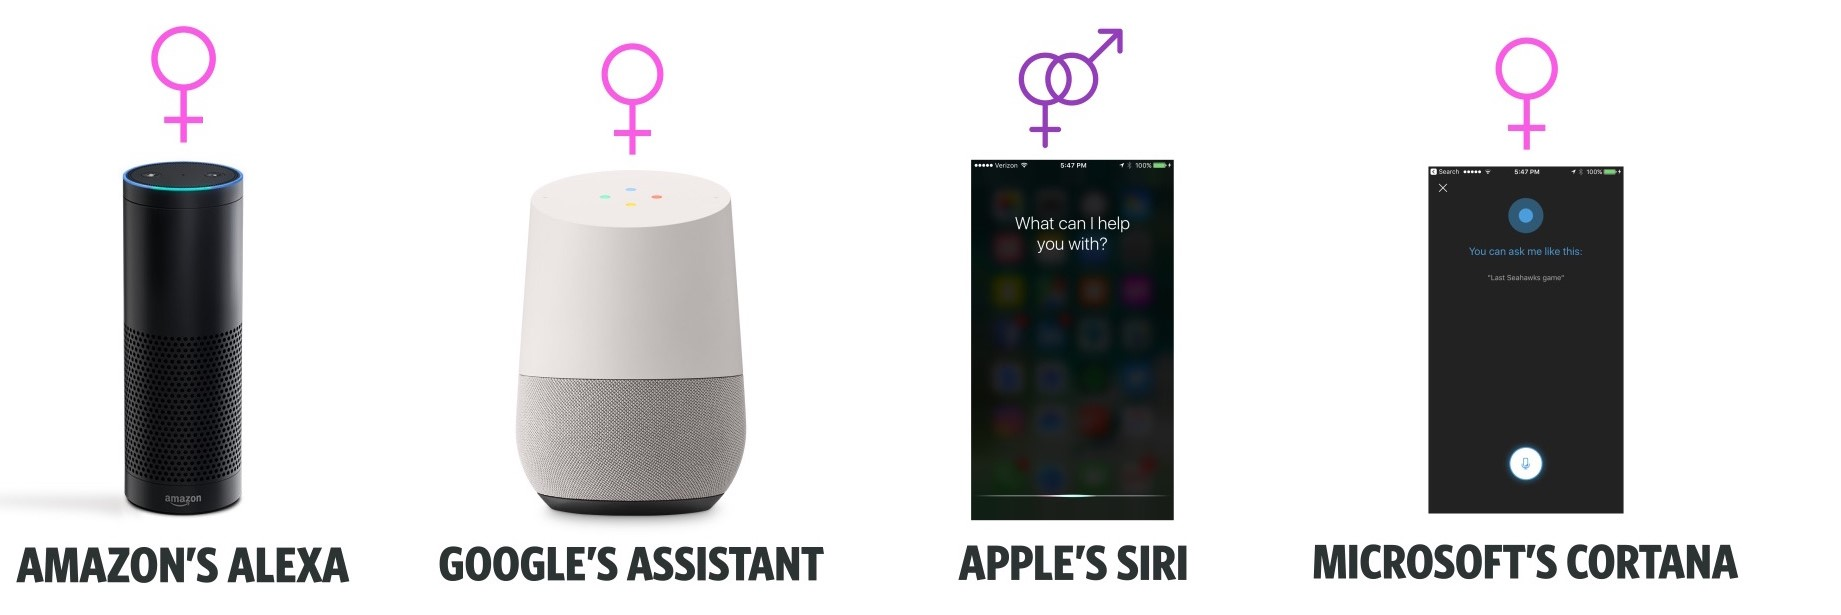
\includegraphics[width=0.9\textwidth]{Images/virtualassistant}
    \caption{Les quatres Assistants Personnels les plus connus - THE WALL STREET JOURNAL}
    \label{fig:mostknownvirtualassistant}
\end{figure}

Les Assistants Personnels sont les IA les plus accessibles pour les consommateurs, leur succès commercial
permet aux entreprises tel que Google, Amazon, Microsoft et Apple d'investir énormément
dans la Recherche et développement.

Pour tout les modèles disponible il faut enoncer une phrase d'activation pour que
l'IA passe en mode écoute, puis donner une commande. Selon les modèles, l'IA
est capable de comprendre le contexte lié de plusieurs questions qui se suivent
comme par exemple le nom du président d'un pays puis son âge, une grande de panoplie de
commandes sont disponible tel que demander des informations sur des commerces et restaurant,
acceder à la domotique connecté de sa maison, lancer des application et s'inscrire à des fils
d'actualité.

Pour ce type de tâches les Assistants Personnels sont encore perfectibles,
la société Loup ventures
\footnote{ Loup Ventures est une société d'investissement en capital risque crée en 2017 et
basé à Minneapolis et new work qui investit dans les technologies de demain. \newline
\url{https://loupventures.com/} }
a effectué une recherche qui se base sur 800 question dans les
catégories suivantes: \newline

\begin{itemize}
    \item Local: ce qui est autour de l'utilisateur (magasins, restaurants et évenements)
    \item Commerce: commander des produits
    \item Navigation
    \item Information: informations de generales ou adapté à l'utilisateur
    \item Commandes: ajouter un rappel, lancer une application, etc. \newline
\end{itemize}

voici les résultats de l'expérience:
\begin{figure}[h]
    \centering
    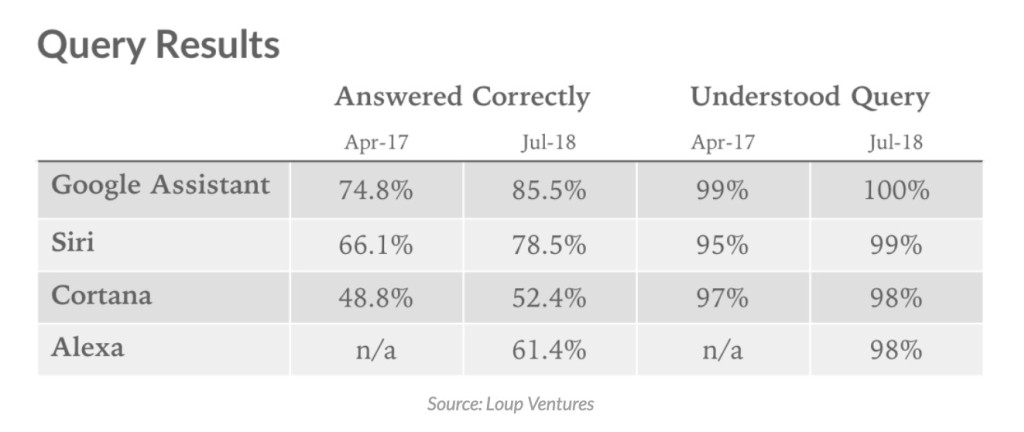
\includegraphics[width=0.8\textwidth]{Images/vaqueryresult}
    \caption{Performances des Assistants Personnels}
    \label{fig:virtualassistantqueryresult}
\end{figure}

On peut voir que les différents Assistants se sont amélioré de 10\% à 20\% d'une année sur l'autre,
de plus le set de questions posées à été changé pour refléter les nouvelles capacités des Assistant
il ne s'agit pas de ce fait d'une amélioration linéaire. Malgré ces résultats les performances
sont assez faibles omissions faite du Google Assistant et pourtant d'un point de vue
humain les question sont extrêmement simple, en effet toute les questions ne sont que des commandes ou
des demandes d'agreggation d'informations, il n'y a qu'une interaction faible avec l'IA qui se révèle
être extrêment basique. Tout les Assistants Personnels sont limités par le nombre de scénarios auxquels
ils peuvent réagir et en effet certaines catégories donnent des résultat bien meilleur que les
autres.

\begin{figure}[H]
    \centering
    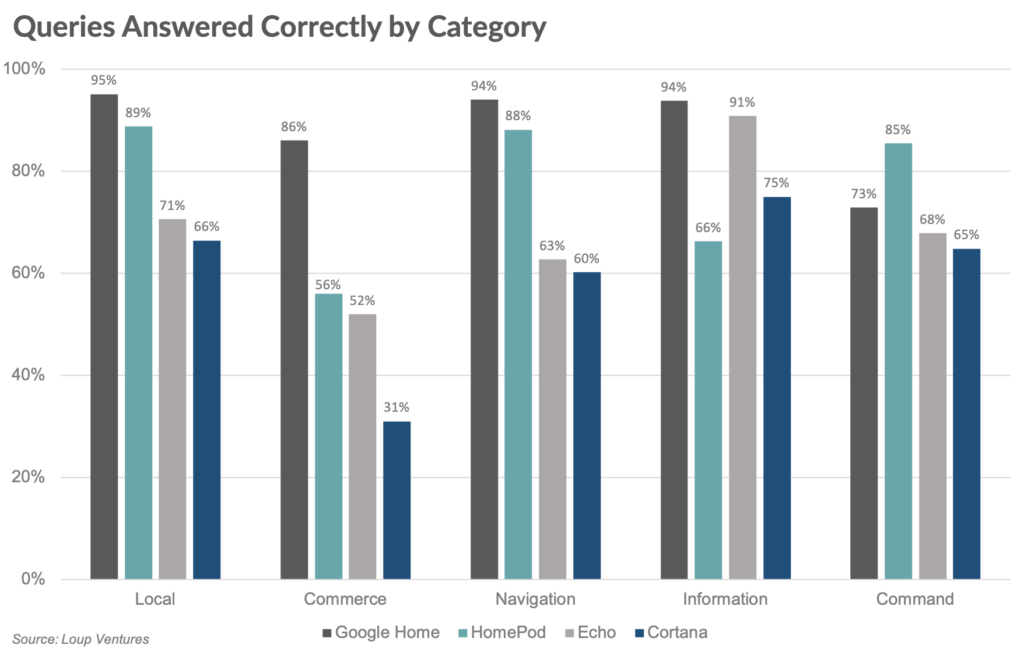
\includegraphics[width=1.0\textwidth]{Images/vaquerybycategory}
    \caption{Résultats par catégories}
    \label{fig:watsonlogo}
\end{figure}

Cependant un problème majeur fait sont apparition: la disparité de performance entre les accents
et les différents langages, en effet tout les tests de performance utilisent l'anglais américain,
le Washington Post ainsi que deux laboratoire de recherche ont étudiés les différence
de précision des assistants virtuels en fonction des accents et langues utilisées, une
perte de précision est visible dès lors qu'un accent autre que l'anglais américain de la Côte Ouest
est utilisé pour google home et autre qu'un accent du Sud pour Amazon Echo. \newline

L'utilisation de plusieurs langue dans une même requête à l'assistant est aussi source 
d'erreur, par exemple avec le google assistant il est bien spécifié dans l'aide 
que ce dernier ne peux comprendre plusieurs langues en même temps or aujourd'hui beaucoup
d'échanges utilisent des mots anglais, si je demande le synopsis d'un film avec 
un titre anglais la prononciation anglaise risque d'induire l'assistant en erreur ce qui
est très problématique dans le domaine professionnel où les termes techniques 
sont majoritairement en anglais indépendement de la langue pratiquée. 



\begin{figure}[H]
    \centering
    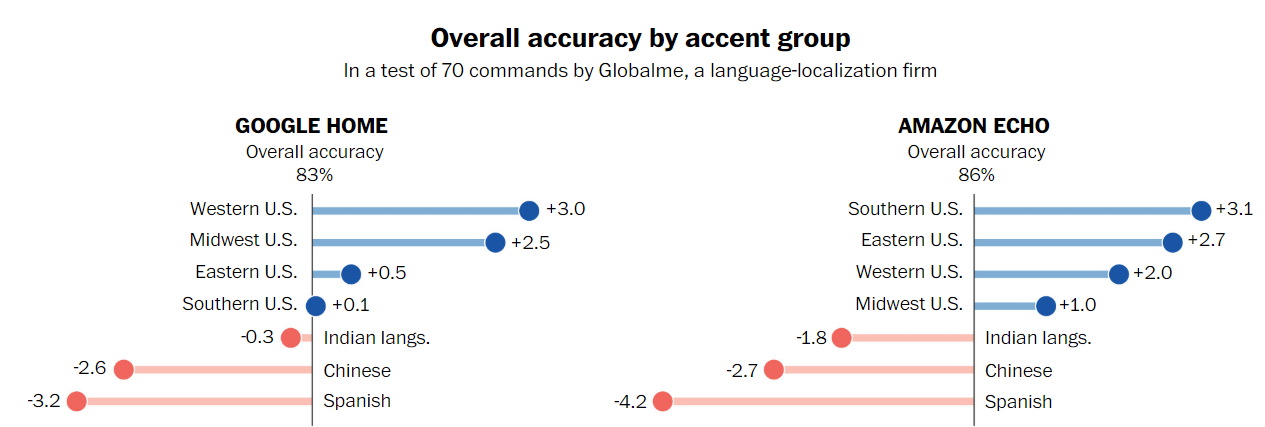
\includegraphics[width=1.0\textwidth]{Images/accuracyperaccent}
    \caption{Précision en fonction des accents - The Washington Post}
    \label{fig:accentaccuracy}
\end{figure}

Les résultats sont intéressant et montre qu'il est important de ne pas seulement se baser sur des
test qui ont été fait exclusivement en anglais, le taux de précision "international" étant
6\% à 10\% plus bas que la réalité et parfois même 30\% plus faible quand il s'agit de quelqu'un
parlant anglais mais n'ayant pas l'anglais comme langue native !\footnote{The Washington Post:
<< People with nonnative accents, however, faced the biggest setbacks. In one study that compared
what Alexa thought it heard versus what the test group actually said, the system showed that speech
from that group showed about 30 percent more inaccuracies>>} \newline

\paragraph{En Conclusion} les Assistants Personnels tel que Google Assistant, Amazon Echo, Siri et
Cortana sont les IA ayants la reconnaissance vocales la plus avancée or les résultat sont toujours
perfectible et il ne s'agit pas d'echanges conversationnel mais toujours de requêtes
ayant pour but une action simple ou une aggrégation de donnée basique, nous sommes très loin
de pouvoir réussir le test de turing et encore plus de réussir à simuler l'intelligence tel que
lors de l'expérience chinese room.


\subsection*{L'IA Watson d'IBM}
\begin{figure}[H]
    \centering
    
\includegraphics[width=0.2\textwidth]{Images/watsonlogo}
    \caption{Avatar de l'ordinateur watson - IBM}
    \label{fig:watsonlogo}
\end{figure}

%petit smalltalk pour représenté watson si jamais deja présenté dans la premiere partie
L'IA Watson a fait de grande vagues lors de sa présentation au publique pour le jeu télévisé jeopardy,
sans-cesse mise en avant cette IA a subit une publicité continue de la part de la société.
Watson est une IA qui a évolué depuis jeopardy en 2011, à cette époque l'IA fonctionnait
par entrainement supervisé avec des donnée fortements méticuleusement traité avant de les utilisé
dans des ensembles de question/réponse très précis, les résultats étaient là mais le coût (il était
nécéssaire d'avoir des développeurs pour pouvoir utiliser la platforme Watson) bien trop élevé.
En 2016 Watson est completement refait à neuf et utilise des \gls{API}s séparant en services
les fonctionnalités de l'IA Watson. \newline

\begin{figure}[H]
    \centering
    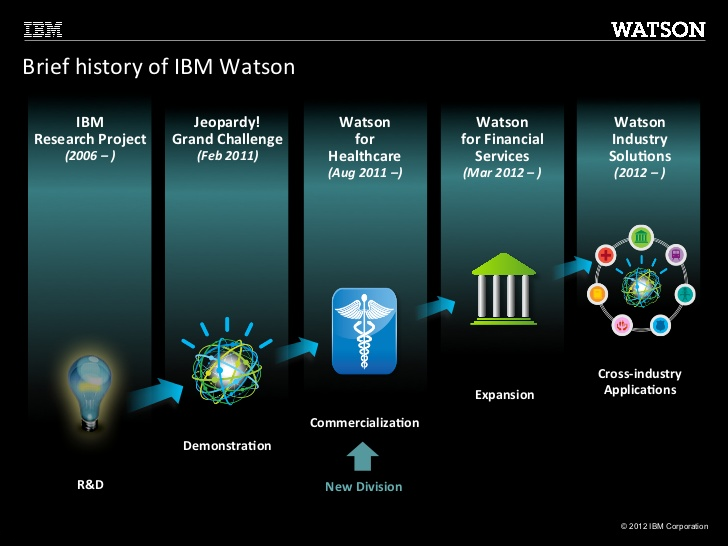
\includegraphics[width=0.7\textwidth]{Images/historyofwatson}
    \caption{Évolution de l'IA Watson - IBM}
    \label{fig:historyofwatson}
\end{figure}


Watson a été présenté comme une IA très puissante dans le domaine de la santé et notamment
celui de la recherche contre le cancer, En 2013 IBM s'associe avec
le Memorial Sloan-Kettering Cancer Centre\footnote{
    le Memorial Sloan-Kettering Cancer Centre est un hopital pour le traitement du cancer situé à new
    york, il a été fondé en 1884 sous le nom de New York Cancer Hospital. \newline
    source: \url{https://en.wikipedia.org/wiki/Memorial_Sloan_Kettering_Cancer_Center}

} pour rassembler des connaissances en
cancerologie et les rendre accessible à l'international sous le service <<Watson for oncology>>
\footnote{\url{https://www.ibm.com/us-en/marketplace/ibm-watson-for-oncology}}. \newline

Watson est aussi utilisé dans le robot Pepper développé par Softbank Robotics:
<<Pepper est le premier robot humanoïde au monde capable d'identifier les visages et
les principales émotions humaines. Pepper a été conçu pour interagir avec
les humains de la façon la plus naturelle possible à travers le dialogue et son écran tactile.>>
\footnote{\url{ source: https://www.softbankrobotics.com/emea/fr/pepper }} \newline

\begin{figure}[H]
    \centering
    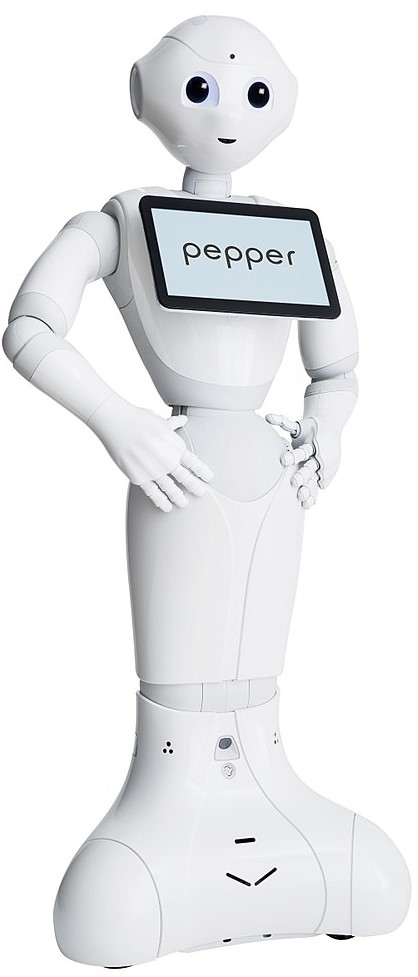
\includegraphics[width=0.2\textwidth]{Images/pepper}
    \caption{Robot Pepper- Softbank Robotics Europe}
    \label{fig:pepperrobot}
\end{figure}

Pepper en tant que projet commercial pilote est un succès avec plus de 12 000 robots vendu en
Europe, le robot étant surtout utilisé en tant que receptionniste dans les entreprises.
\footnote{\url{https://www.forbes.com/sites/parmyolson/2018/05/30/softbank-robotics-business-pepper-boston-dynamics/\#60bc31464b7f}}
\newline
Malgré watson et pepper, le succès semble relatif voir meme plus négatif qu'IBM ne semble laisser paraître,
en effet en Février 2017 le MD Anderson Cancer Center\footnote{\url{https://www.mdanderson.org/}}
qui avait décidé en 2013 d'utiliser Watson pour assister les practiciens pour le traitements
du cancer, a stoppé le projet indiquant une absence de résultat dû à plusieurs facteurs:
\footnote{Source: Rapport d'Audit publié par le University of Texas Audit Office
    \url{https://www.utsystem.edu/sites/default/files/documents/UT\%20System\%20Administration\%20Special\%20Review\%20of\%20Procurement\%20Procedures\%20Related\%20to\%20UTMDACC\%20Oncology\%20Expert\%20Advisor\%20Project/ut-system-administration-special-review-procurement-procedures-related-utmdacc-oncology-expert-advis.pdf}}
\newline

\begin{itemize}
    \item Le projet de départ était estimé à 5 millions de dollars, lors de l'arrêt du
    projet, MD Anderson avait dépensé 62 millions de dollars sur l'Oncology
    Expert Advisor utilisant entre autres des fond de donateurs pas encore reçus. \newline

    \item Le projet a été approuvé sans l'accord de la direction du
    département informatique tel que le procédure standard l'exige, de plus il y a
    eu un manque de transparence dans la majorité des taches administratives et
    financières du projet: il s'agit de gros problèmes de management qui ont conduit
    à l'echec du projet.\newline

    \item OEA n'est pas compatible avec le logiciel EHR
    \footnote{
        EHR = Electronic Health Record, il s'agit du dossier médical digital d'un patient.
    } utilisé par MD Anderson, EPIC, alors qu'IBM avait la connaissance du changement
    de logiciel et a même lancé une collaboration avec EPIC pour être compatible
    et 14 centres de recherche dans lequel utiliser leur partenariat,
    MD Anderson ne faisait pas partie de ces 14 etablissements
    \footnote{
        \url{https://www.healthcareitnews.com/news/epic-watson-work-interoperability}
    } ce qui a pour effet de rendre tout le projet OEA inutilisable.
    \newline

    \item IBM a présenté AOE comme une solution miracle, avec tout le travail
    de publicité et de marketing pour pousser cette narrative, alors qu'ils n'ont
    pas été capable de comprendre et répondre correctement au besoin des cancerologues:
    en effet une des lignes directrices du produit AOE est la capacité à centraliser
    et analyser des centaines voir milliers de publication scientifiques sur la
    recherche sur le cancer pour aider le cancerologue sur le choix de traitements
    or comme le dit David Howard\footnote{\url{https://www.healthnewsreview.org/2017/02/md-anderson-cancer-centers-ibm-watson-project-fails-journalism-related/}}
    <<le problème n'est pas la saturation de publications scientifiques
    que les practiciens n'ont pas le temp de lire mais le peu de publications
    de qualité et réelement utile à ce dernier>>. \newline
\end{itemize}

\begin{figure}[H]
    \centering
    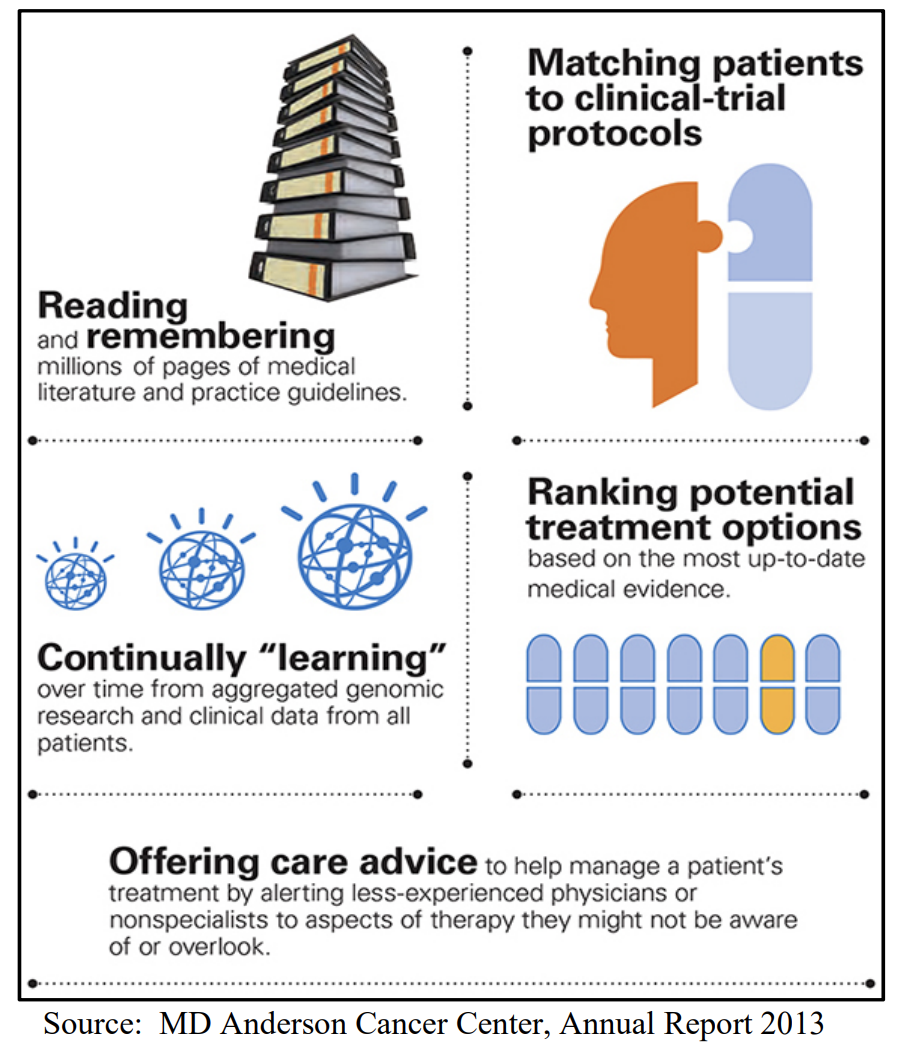
\includegraphics[width=0.6\textwidth]{Images/mdanderson}
    \caption{les caractéristiques de l'Oncology Expert Advisor}
    \label{fig:mdanderson}
\end{figure}

\paragraph{En Conclusion} l'IA n'est qu'une solution, et la structure qui l'entoure est
tout aussi importante car la mise en place de logiciel utilisant la puissance de
l'Intelligence Artificelle n'est pas aisé car il faut identifier le besoins et les contraintes,
ce que l'on cherche à résoudre de manière bien plus précise qu'avec des algorithmes
traditionnels, le projet de l'Oncology Expert Advisor au sein du centre
MD Anderson est l'exemple parfait d'une mauvaise structure (mauvaise gestion de projet)
ainsi qu'une mauvaise interprétation du besoin de la part d'IBM qui a surtout
chercher à se faire de la publicité plutôt qu'a réellement résoudre des problèmes.

\subsection*{Deepmind}
\begin{center}
    
\includegraphics[width=0.4\textwidth]{Images/deepmindlogo}
\end{center}

DeepMind Technologies est une entreprise britannique fondé en 2010 qui a été
racheté par Alphabet Inc, la maison mère de Google. \newline

<<L’objectif de DeepMind est de "résoudre l'intelligence". Pour atteindre ce but,
l'entreprise essaie de combiner "les meilleures techniques de l'apprentissage automatique et
des neurosciences des systèmes pour construire de puissants algorithmes d'apprentissage généraliste".
L'entreprise souhaite non seulement doter les machines d'intelligence artificielle performante,
mais aussi comprendre le fonctionnement du cerveau humain. >>
\footnote{\url{https://fr.wikipedia.org/wiki/DeepMind}} \newline

L'entreprise utilise des IA capables d'apprendre à jouer à des jeux vidéos ou l'extrêmement complexe
jeu de Go, en effet une IA avec une intelligence proche de l'homme serait capable d'apprend à jouer
à n'importe quel jeu en se basant seulement sur des stimuli visuel et/ou tactile. Deepmind utilise
la perception visuelle dans ses IA, le but est d'utiliser les données les plus brut possible,
au contraire de beaucoup d'IA où la géneration de feature est extrêmement poussé rendant l'IA
dépendante du raffinement des features définies, ainsi que les connaissances acquis lors de l'entraînement
sur les jeux joués précédement. \newline

Pour réussir un tel exploit DeepMind utilise l'Apprentissage Profond Renforcé:

\begin{figure}[H]
    \centering
    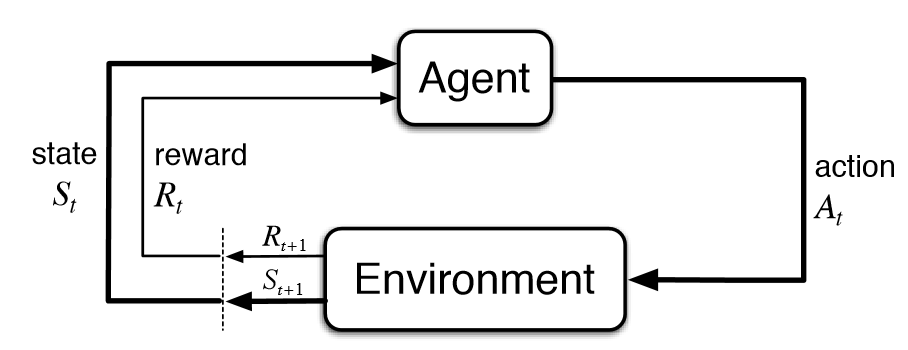
\includegraphics[width=0.5\textwidth]{Images/reinforceddeeplearning}
    \caption{apprentissage profond renforcé - towardsdatascience}
    \label{fig:reinforceddeeplearning}
\end{figure}

L'apprentissage profond renforcé ou Reinforced Deep Learning est un dérivé de l'apprentissage
renforcé appartenant au domaine du machine learning concernant comment un agent intelligent
\footnote{<<En intelligence artificielle, un agent intelligent (AI) est une entité autonome capable de
percevoir son environnement grâce à des capteurs et aussi d'agir sur celui-ci via des effecteurs
afin de réaliser des buts.
Un agent intelligent peut également apprendre ou utiliser des connaissances pour pouvoir réaliser
 ses objectifs. Les agents intelligents sont souvent décrit schématiquement comme des systèmes fonctionnels abstrait
similaire au logiciels informatique. Certaines définition mettent en avant leur autonomie
et vont donc préférer le terme agent intelligent autonome>> \newline
source: \url{https://fr.wikipedia.org/wiki/Agent_intelligent} \newline},
agent intelligent autonome plus précisement, peut atteindre un objectif de manière itérative en
interagissant avec l'environnement avec la meilleure performance possible. \newline

Contrairement au deep learning qui se base sur un set de données d'entraînement
puis est utilisé sur de nouvelles données, un algorithme d'apprentissage profond
s'entraîne et s'améliore continuellement en utilisant les données qui lui sont
fournis. \newline

Une des autres différences entre le Deep Learning et le Reinforced Learning
(qu'il soit composé d'un réseau de neurone ou non) est la différence des résultats,
dans le cas du Reinforced Learning le resultat obtenu en fonction des décisions
prises est partiellement aléatoire ou du moins ne peut être determiné dans un ensemble finis
et prédéfinis à l'avance comme c'est le cas avec un algorithme de deep learning,
de plus le résultat attendu peut ne pas se présenter immédiatement et arriver
qu'après un nombre aléatoire d'action puisque l'agent intelligent autonome qui utilise
l'apprentissage renforcé agis sur l'environnement qui est lui même la source de
ses entrée, ses actions peuvent l'éloigner du résultat attendu contrairement
au deep learning ou la rétropropagation
\footnote{<< la rétropropagation du gradient est une méthode pour calculer le gradient de l'erreur
pour chaque neurone d'un réseau de neurones, de la dernière couche vers la première.
De façon abusive, on appelle souvent technique de rétropropagation du gradient l'algorithme classique
de correction des erreurs basé sur le calcul du gradient grâce à la rétropropagation et
c'est cette méthode qui est présentée ici. En vérité, la correction des erreurs peut se faire selon
d'autres méthodes, en particulier le calcul de la dérivée seconde. Cette technique consiste à corriger
les erreurs selon l'importance des éléments qui ont justement participé à la réalisation de ces erreurs.
Dans le cas des réseaux de neurones, les poids synaptiques qui contribuent à engendrer une
erreur importante se verront modifiés de manière plus significative que les poids qui ont engendré
une erreur marginale.>> \newline
Source: \url{https://fr.wikipedia.org/wiki/Rétropropagation_du_gradient}}
impacte la manière dont les entrée
sont traitées mais pas les entrées elles-même, on peu faire de manière abstraite un rapprochement
entre logique et machine learning où le Deep Learning serait la logique combinatoire et
l'apprentissage renforcé la logique séquentielle. \newline

Le Reinforced Learning se rapproche de part son fonctionnement de la réflexion humaine en faisant 
des inférences à partir d'informations partielles, l'illustration simple de se principe 
dans la vrai vie est celle du vent et des feuilles qui bougent: 
on observe des feuilles d'arbres qui bougent et par inférence sans même vérifier s'il y a du 
vent ont en déduit qu'il y a présence de vent. 

\paragraph{En Conclusion} Deepmind utilise des technologies très avancées mais 
ne fait au final qu'office de vitrine de publicité de la recherche et du développement 
de DeepMind Inc et Google plutôt que d'avoir un produit commercialisable. 


\newpage
\section{La problématique de l'automatisation des métiers}
%il y a 2 segments de problemes (conclusion de la partie précédente):
% - Le coût et la gestion de projet/management (ex: watson)
% - Les performances réel (ex: assistants virtuels)

\subsection*{Tout les métiers ne sont pas automatisables}
\subsection*{La resistance au changement forte avec l'IA}
%utiliser https://www.inc.com/thomas-koulopoulos/its-time-to-stop-calling-it-artificial-intelligence.html
% comme support d'argumentation